%!TEX root = ../main.tex

\teaser{
	\plaatje{Voeg phong tesselation model toe.}
	
	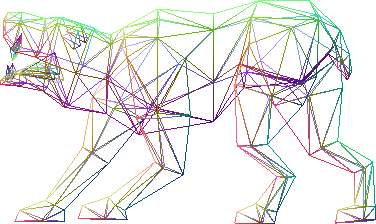
\includegraphics[width=0.3\linewidth]{content/img/header/dogWireFrame.png}
	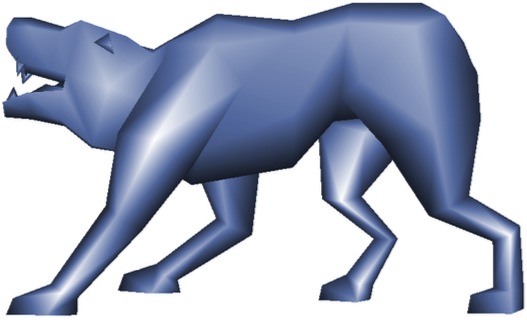
\includegraphics[width=0.3\linewidth]{content/img/header/dogModel.png}
	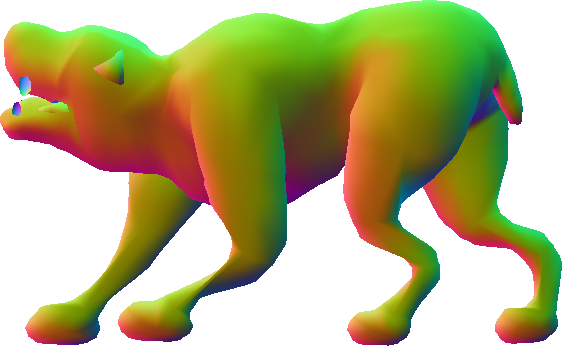
\includegraphics[width=0.3\linewidth]{content/img/results/dogGPU.png}
	\centering
	\caption{From left to right, the input triangulation, the model, and the curved point-normal model, colored according to its normals.}
	\label{fig:preamble:teaser}
}

\maketitle